\chapter{Fazit und Ausblick}
\label{ch:Ausblick}

Zum Abschluss wird in diesem Kapitel über die Arbeit reflektiert und diskutiert wie ein solches Projekt weitergeführt werden könnte und welche Verbesserungs- oder Erweiterungsmöglichkeiten es gibt.

\section{Technisches Fazit}

Technisch wurden die Anforderungen erfüllt. Leider ist es jedoch nicht gelungen ein System zu entwickeln, welches hundertprozentig zuverlässig Personen von anderen Wärmequellen unterscheiden kann. Das \gls{CNN} ist darin zwar besser als die Threshold Methode, leider kann es aber auch nicht in allen Fällen korrekt entscheiden, es erzielte in den Tests eine Präzision von 93\%. Dieses Problem könnte durch Training mit mehr Daten und/oder mehr, und spezifischeren Klassen minimiert werden.

\section{Projektfazit}

Das Projekt war rückblickend gesehen erfolgreich. Auch wenn das entwickelte System nicht mit hundertprozentiger Genauigkeit arbeitet, konnte gezeigt werden, wo die Herausforderungen liegen und was getan werden kann, um diese zu meistern. Es wurde gezeigt, dass das Erkennen von Personen relativ einfach ist, das Unterscheiden von Personen von anderen Wärmequellen hingegen eine Herausforderung darstellt. Da bei so kleiner Auflösung sehr wenig Information zur Verfügung steht und Personen viele verschiedene Haltungen einnehmen können (siehe Abbildung \ref{fig:postureExample}), ist es schwierig ein perfektes Modell dazu zu erstellen.

\begin{figure}[H]
	\centering
	\begin{subfigure}{.4\linewidth}
		\centering
		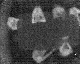
\includegraphics[keepaspectratio, height=4cm]{postureExample1}
	\end{subfigure}
	\begin{subfigure}{.4\linewidth}
		\centering
		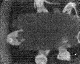
\includegraphics[keepaspectratio, height=4cm]{postureExample2}
	\end{subfigure}	
	\caption{Beispielbilder Haltung}
	\label{fig:postureExample}
\end{figure}

\subsection{Persönliches Fazit}

Ich sehe das Projekt auch persönlich als einen Erfolg an. Ich werde bestimmt viele Dinge mitnehmen, die ich während des Projekts gelernt habe. Natürlich verlief auch in diesem Projekt nicht immer alles nach Plan und ich musste Zeit in die Lösung von Problemen investieren, die nicht direkt das System betrafen. Doch alles in allem konnte ich ein funktionierendes System entwickeln, welches mit einer 92\% Sicherheit und 93\% Präzision Personen erkennt und deren Position bestimmen kann.

\section{Ausblick}
Um dieses Projekt erfolgreich weiterzuführen und auszubauen, könnte man das \gls{CNN} durch einen grösseren Trainingsdatensatz von mindestens 1000 Bildern jeder Klasse verbessern. Auch wäre es angebracht zu evaluieren, ob mehr und spezifischere Klassen sinnvoll wären. Die momentane Fremde-Wärmequellen-Klasse beinhaltet sehr verschiedene Objekte, wie Laptops, Kaffees oder die erwärmte Fensterbank. Würde man dies feiner granulieren, könnte das \gls{CNN} sie besser erkennen.\\
Die Threshold-Methode hingegen bietet kaum Optimierungspotenzial. Man könnte einzig noch umgebungsspezifische Anpassungen vornehmen. Zum Beispiel könnte die Fensterbank oder der Bereich des Sitzungstisches ausgeschlossen werden. Diese Methode ist jedoch sehr anfällig auf Änderungen im Raum. Wird beispielsweise der Tisch verschoben, funktioniert der Algorithmus nicht mehr korrekt. Auch wäre dadurch der Einsatz in einer anderen Umgebung nicht ohne grössere Änderungen des Algorithmus möglich. Sollte dieses System in einer anderen Umgebung eingesetzt werden, muss evaluiert werden, ob die Vogelperspektive der Kamera die richtige Wahl ist. Sollte dies nicht der Fall sein müsste das CNN mit komplett neuen Trainingsdaten trainiert werden. Auch die Threshold-Methode müsste sehr wahrscheinlich überarbeitet werden.
